\section{Methodology}
\label{sec:method}
% include the figures path relative to the master file
\graphicspath{ {./content/method/figures/} }

% \begin{figure}[t]
%     \centering
%     \begin{subfigure}[b]{0.30\textwidth}
%         \centering
%         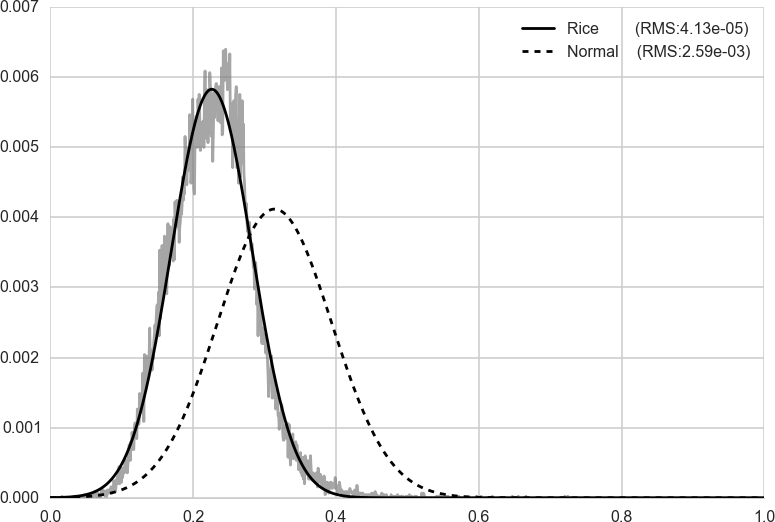
\includegraphics[width=\textwidth]{03}
%     \end{subfigure}
%     \hfill
%     \begin{subfigure}[b]{0.30\textwidth}
%         \centering
%         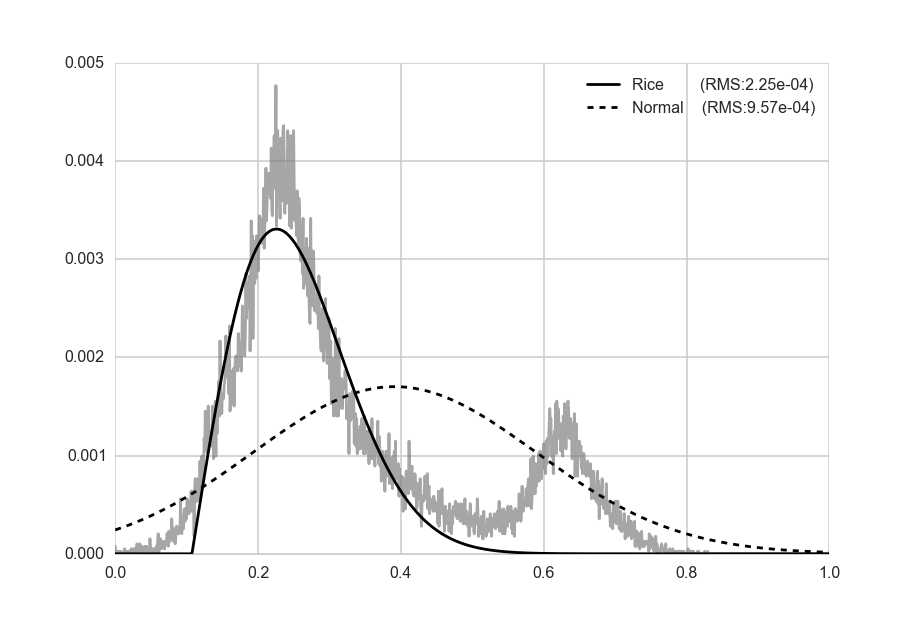
\includegraphics[width=\textwidth]{06}
%     \end{subfigure}
%     \hfill
%     \begin{subfigure}[b]{0.30\textwidth}
%         \centering
%         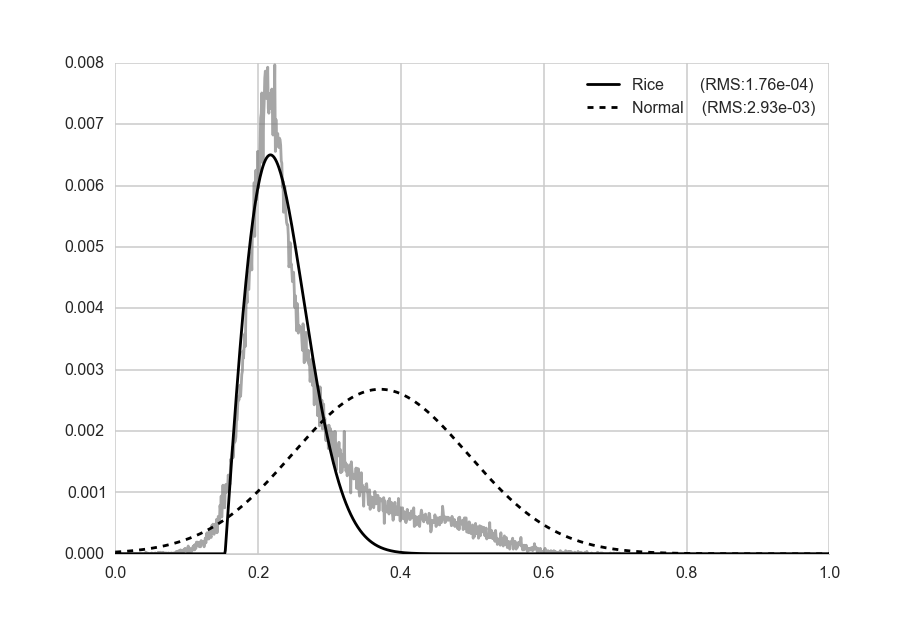
\includegraphics[width=\textwidth]{14}
%     \end{subfigure}
%     \caption {Fitting differences}
%     \label{fig:rice-norm-diff}
% \end{figure}

As stated in~Sect.\,\ref{sec:descr} proper normalization of the \ac{mri} data during pre-processing is a key problem that has been addressed from a parametric and non-parametric point of view.
We believe that normalizing \ac{mri} data using a parametric model based on Rician distribution would improve the results for the parametric case.
Expecting this improvement by changing the data model from Gaussian to Rician distribution is reasonable since Bernstein~\emph{et al.}\,\cite{bernstein1989improved} statet that \ac{mri} data follows a Rayleigh distribution for low \ac{snr} scenarios while it appears closer to a Gaussian distribution when \ac{snr} increases.
Figure~\ref{fig:fitting} shows the intensity spectrum for some \ac{mri} prostate data.
A qualitative assessment of the underlying distribution is done by overlying the resulting distribution of fitting the entire data.
Quantitative results of the fitting are given in terms of \ac{rms}.

\begin{figure*}
  \centering
  \subfloat[][]{
    \label{fig:p1}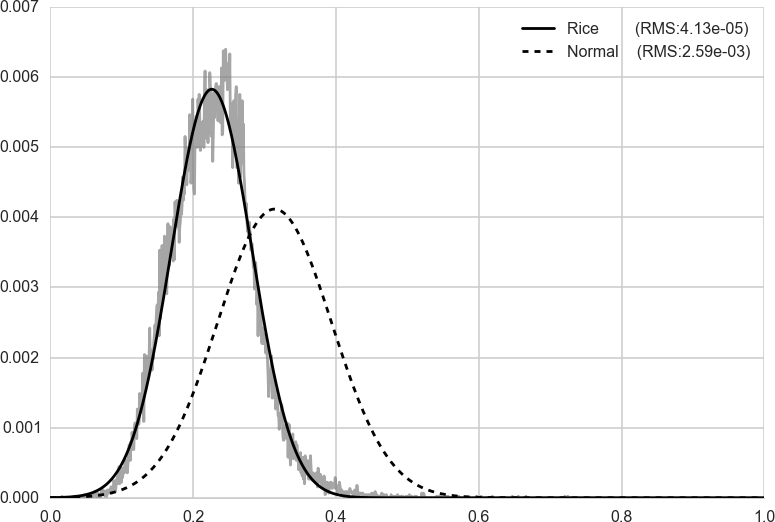
\includegraphics[width=0.3\textwidth]{03}}\hfill
  \subfloat[][]{
    \label{fig:p2}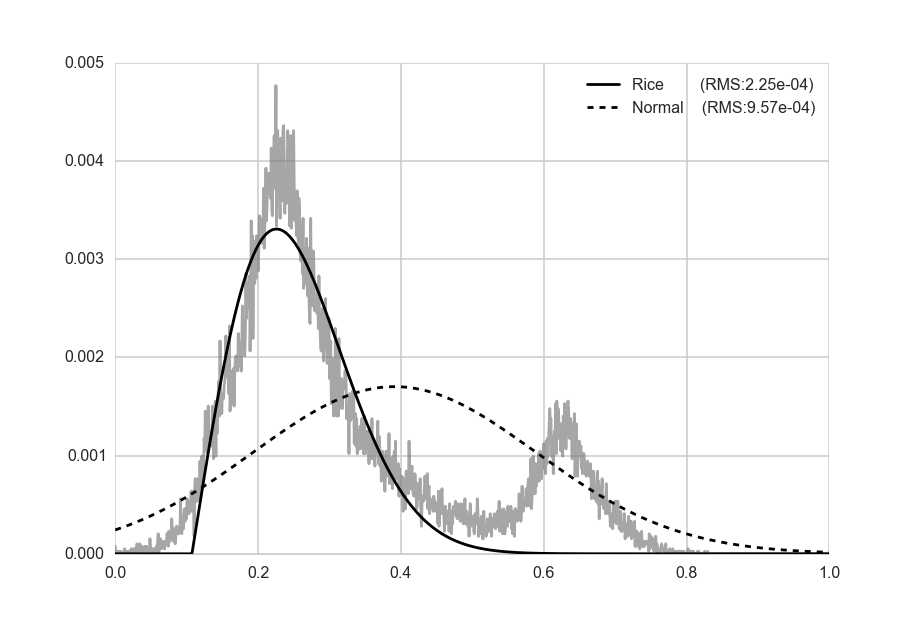
\includegraphics[width=0.3\textwidth]{06}}\hfill
  \subfloat[][]{
    \label{fig:p3}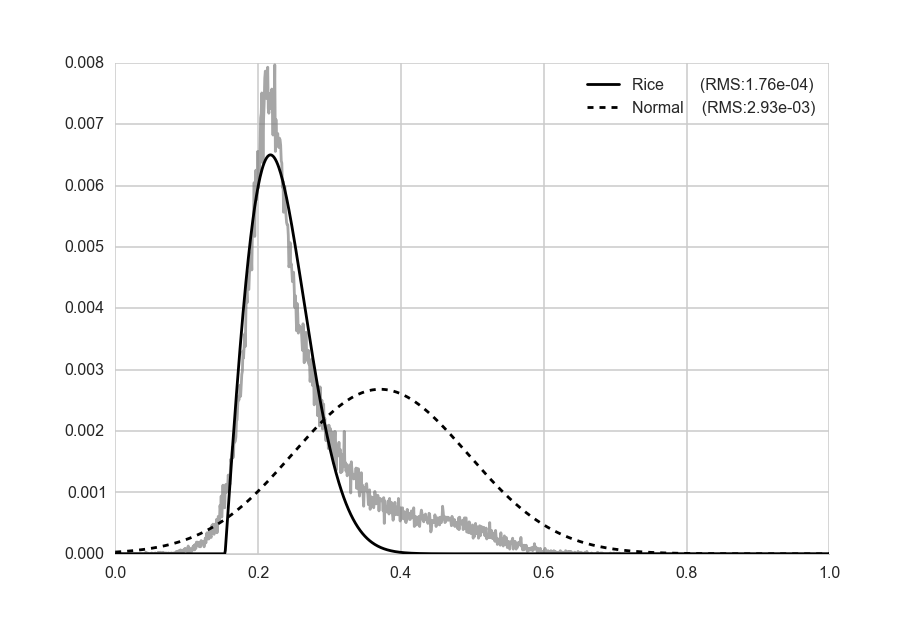
\includegraphics[width=0.3\textwidth]{14}}
  \caption{Visual evaluation of the goodness of fitting using Rician and Gaussian distribution.}
  \label{fig:fitting}
\end{figure*}


%%% Local Variables: 
%%% mode: latex
%%% TeX-master: "../../master"
%%% End: 

